\documentclass{article}

\usepackage[main=english,vietnamese]{babel}
\usepackage[T1]{fontenc}
\usepackage[utf8]{inputenc}
\usepackage[sexy]{evan}
\usepackage{matchsticks}
\usepackage{wrapfig}
\usepackage{listings}

\newtheorem{hint}{Hint}

\title{Eight ways to prove - Part 2}
\author{Nghia Doan}
\date{\today}

\begin{document}

\maketitle

This article is the second part of the series on explore different topics of geometry to find a way for the same problem.

\begin{example*}[IMO 2014, Problem 4]
    Let $P$ and $Q$ be on segment $BC$ of an acute triangle $ABC$ such that $\angle PAB=\angle BCA, \angle CAQ=\angle ABC.$
    Let $M$ and $N$ be points on lines $AP$ and $AQ,$ respectively, such that $P$ and $Q$ are midpoints of $AM$ and $AN,$ respectively.
    Prove that the intersection $S$ of $BM$ and $CN$ is on the circumference of $\triangle ABC$.    
\end{example*}

\begin{theorem*}[Pascal's Theorem]
    \label{theorem:pascal-theorem}
    Let $\mathcal{P}=A_1A_2A_3A_4A_5A_6$ be a hexagon,
    $C_1 = A_1A_2 \cap A_4A_5$, $C_2 = A_2A_3 \cap A_5A_6$, $C_3 = A_3A_4 \cap A_6A_1$.
    Then $\mathcal{P}$ is a cyclic hexagon (which is circumscribed by a circle)
    if and only if $C_1, C_2, C_3$ are collinear.
\end{theorem*}

\begin{center}
    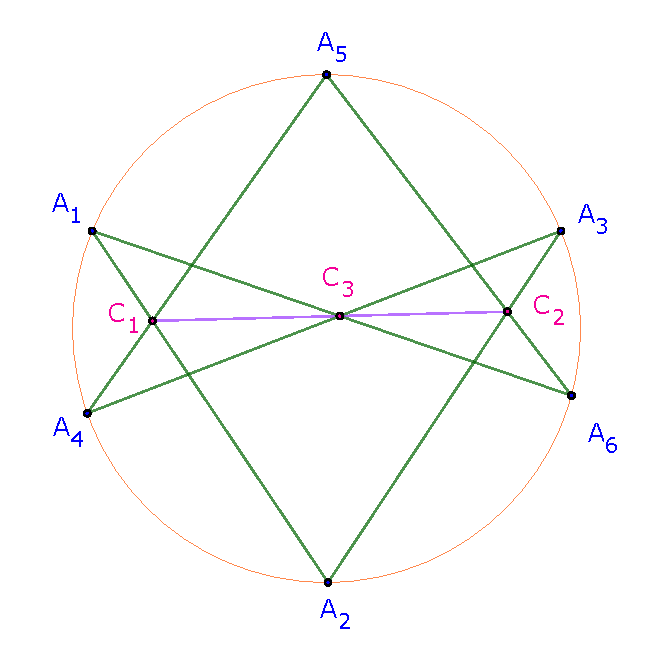
\includegraphics[width=6.5cm]{./svg/pdf/pascal-theorem.pdf}
\end{center}

\newpage

\begin{proof}[\textbf{$5^{\text{th}}$ proof based on \nameref{theorem:pascal-theorem}}]
    Let $\Omega$ denote the circle. Let points $L = \Omega \cap AN,$ $K = \Omega \cap AM.$
    Since $\angle LBC = \angle LAC = \angle CBA$ and $\angle KCB = \angle KAB = \angle BCA,$
    thus $X = BL \cap CK$ is an image of $A$ by the reflection over the line $BC.$

    \begin{center}
        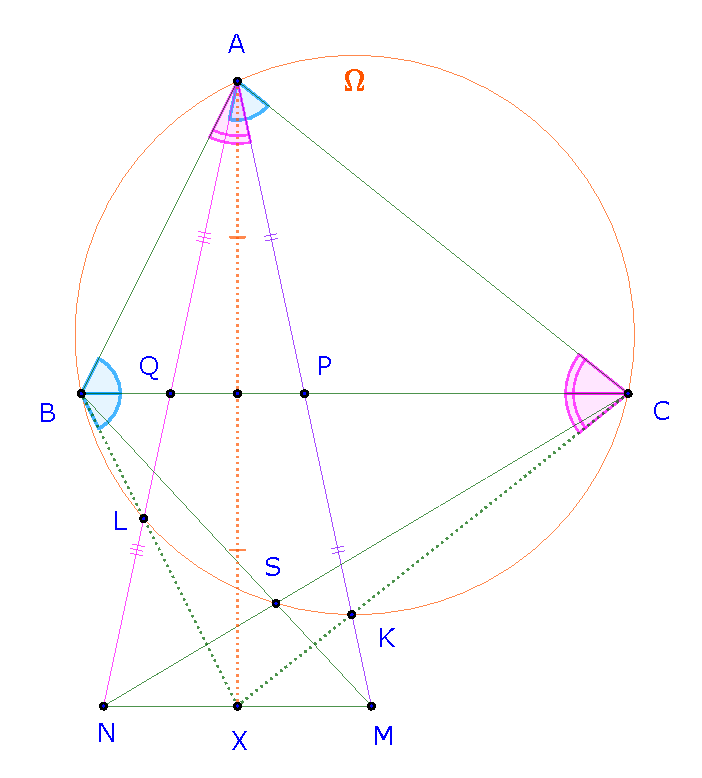
\includegraphics[width=7.5cm]{./svg/pdf/ot-22-23-4-e2-s3.pdf}
    \end{center}

    Since $Q$ and $P$ are midpoints of $AN$ and $AM,$ so $X$ must be on $NM$.
    Thus if $\mathcal{P}=A_1A_2A_3A_4A_5A_6$ denotes $ALBSCK,$
    then since $N = AL \cap SC,$ $X = LB \cap CK,$ and $M = BS \cap KA$ are collinear
    thus $ALBSCK$ is cyclic. Therefore $S$ is on the circle $(ABC).$
\end{proof}

\newpage

\begin{proof}[\textbf{$6^{\text{th}}$ proof based on the Law of Sines}]
    First $\angle PAB = \angle BCA = \angle C,$ $\angle CAQ = \angle ABC = \angle B.$
    Thus $\triangle PBA \sim \triangle QAC \sim \triangle ABC.$
    
    \begin{center}
        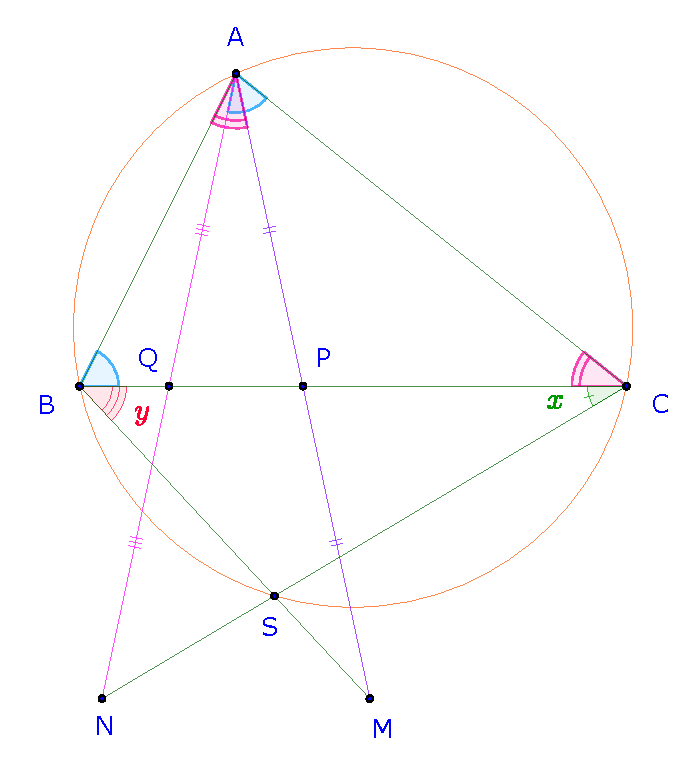
\includegraphics[width=7.5cm]{./svg/pdf/ot-22-23-4-e2-s4.pdf}
    \end{center}
    
    By the Law of Sines for $\triangle QCN,$ and note that $\angle QNC = \angle AQC - x = \angle A - x,$
    \[
        \begin{aligned}
            \frac{QN}{QC} = \frac{\sin{\angle QCN}}{\sin{ \angle QNC}} = \frac{\sin{x}}{\sin{(\angle A - x)}},\ QN = QA,\ \frac{QA}{QC} = \frac{AB}{AC}
            \Rightarrow \frac{AB}{AC} = \frac{QA}{QC} = \frac{QN}{QC} = \frac{\sin{x}}{\sin{(\angle A - x)}} \quad (1)
        \end{aligned}
    \]

    Similarly for $\triangle PBM, $ $\dfrac{AC}{AB} = \dfrac{\sin{y}}{\sin{(\angle A - y)}} \quad (2).$
     
    From (1) and (2), and note that $\sin{\alpha} \sin{\beta} = \frac{1}{2} \left( \cos{(\alpha - \beta)} - \cos{(\alpha + \beta)} \right),$
    \[
        \begin{aligned}
            &1 =  \frac{AB}{AC} \cdot \frac{AC}{AB} = \frac{\sin{x}}{\sin{(\angle A - x)}} \cdot \frac{\sin{y}}{\sin{(\angle A - y)}}
            \Rightarrow \sin(\angle A-x)\sin(\angle A-y) = \sin{x} \sin{y} \\
            \Rightarrow\ &\cos{(y-x)} - \cos{(x+y- 2 \angle A)} = \cos{(x-y)} - \cos{(x+y)}
            \Rightarrow \cos{(2 \angle A - (x+y))}  = \cos{(x+y)}  \quad (3)
        \end{aligned}
    \]

    Since $x< \angle A, y<\angle A$ and $\cos{\alpha} = \cos{(-\alpha)},$\
    \[
        (3) \Rightarrow 2A - (x+y) = x+y \Rightarrow x+y = A \Rightarrow \angle BSC = 180\dg - \angle A.
    \]

    Therefore $ABSC$ is cyclic and $S$ is on the circle $(ABC).$
\end{proof}

\newpage

\begin{proof}[\textbf{$7^{\text{th}}$ proof based on Analytical Geometry}]
    Let $A(2,0),$ $B(-2b,0),$ $C(2c,0),$ $P(2p,0)$ ($0< b < p < c$) be the coordinates.
    Let $A,$ $B,$ $C$ be the measures of the $\angle A,$ $\angle B,$ $\angle C,$ respectively;
    \begin{center}
        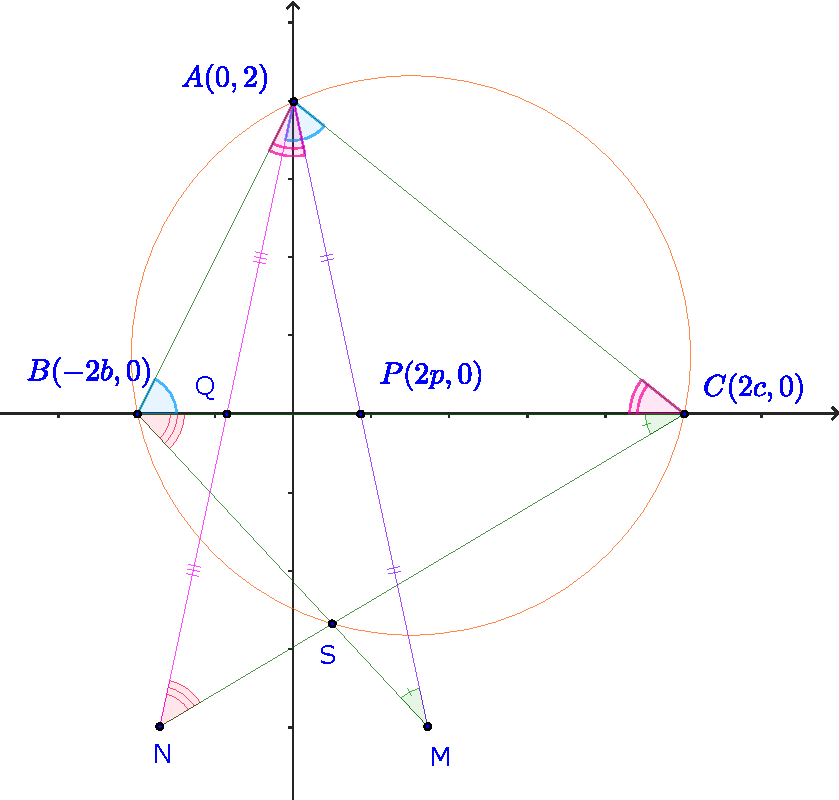
\includegraphics[width=7.5cm]{./svg/pdf/ot-22-23-4-e2-s7.pdf}
    \end{center}
    \[
        \begin{aligned}
            &\cot{B} = \frac{OB}{OA} = b, \cot{C} = c, \cot{A} = \cot{(180\dg-B-C)} = -\cot{(B+C)} = \frac{1-bc}{b+c}\\
            &\frac{PO}{AO} = \cot{A} \Rightarrow p = \cot{\angle APB} = \frac{1-bc}{b+c},
            \Rightarrow P \left( \frac{2(1-bc)}{b+c}, 0\right),\ Q \left(\frac{-2(1-bc)}{b+c}, 0\right),\\
            &P,\ Q \text { are midpoints of } AM,\ AN
            \Rightarrow M \left( \frac{4(1-bc)}{b+c}, 2\right),\ N \left( \frac{-4(1-bc)}{b+c}, -2\right).
        \end{aligned}
    \]
    
    The slope of line $BM$ is $\dfrac{2 - 0}{\dfrac{4(1-bc)}{b+c} - (-2b)} = \dfrac{b+c}{b^2-bc+2}.$
    The equation of line $BM$ is 
    \[
        y - 0 = \left( \frac{b+c}{b^2-bc+2} \right) x - (-2b)
        \Rightarrow y = \left( \frac{b+c}{b^2-bc+2} \right) x + \frac{2b(b+c)}{b^2-bc+2}.
    \]

    Let $D$ be the circumcentre of $(ABC).$ $D_x = \frac{1}{2}(B_x+C_x) =\dfrac{2c+(2b)}{2}=c-b.$
    Line $AC$ is $y=-\dfrac{1}{c}x+2$ the perpendicular bisector of $AC$ has the slope $c$ and
    is through $(c,1).$ Thus, its equation of is $y=cx+(1-c^2).$
    Therefore $D_y=c(c-b)+(1-c^2) = 1-bc.$
    Furtheremore, the circumradius of $(ABC)$ is:
    \[ 
        R = \frac{AB \cdot BC \cdot CA}{4[ABC]} = \frac{2\sqrt{1+b^2} \cdot (2c-2b) \cdot 2\sqrt{1+4^2} }{4 \cdot \frac{1}{2}(2)((2c-2b)) }
        = \sqrt{(1+b^2)(1+c^2)}.
    \]

    Thus, the equation of the circumcircle $(ABC)$ is $\left[ x - (c-b) \right]^2 + \left[ y - (1-bc) \right]^2 = (1+b^2)(1+c^2).$
    It is easy to verify that the intersection of $BM$ with $(ABC)$ is the same as the intersection of $CN$ with $(ABC),$ which is
    point $S$ with coordinates symmetric in regards to $b$ and $c,$
    \[
        S \left( 2\frac{(c-b)(2-bc)}{(c-b)^2+4}, -2\frac{(c+b)^2}{(c-b)^2+4} \right)
        \Rightarrow S = BM \cap CN \in (ABC)
    \]
\end{proof}

\newpage

\begin{proof}[\textbf{$8^{\text{th}}$ proof based on Complex Numbers}]
    Let $X = a+ib$ complex number is represented by a point $X(a,b)$ on the complex plane.
    In short, we write $X,$ and interpret it as both complex number and a number on the complex plane
    (of course depending on what context).

    Note that for points $X, Y$ on the complex plane then $X-Y$ is the \textit{directed} distance of them
    (It is easy to derive by denote $X(x_1, x_2),\ Y(y_1,y_2)$ then $(X-Y)(x_1-x_2,y_1-y_2)$.)
    Also note that $\overline{X}$ is the conjugate of $X.$

    \begin{center}
        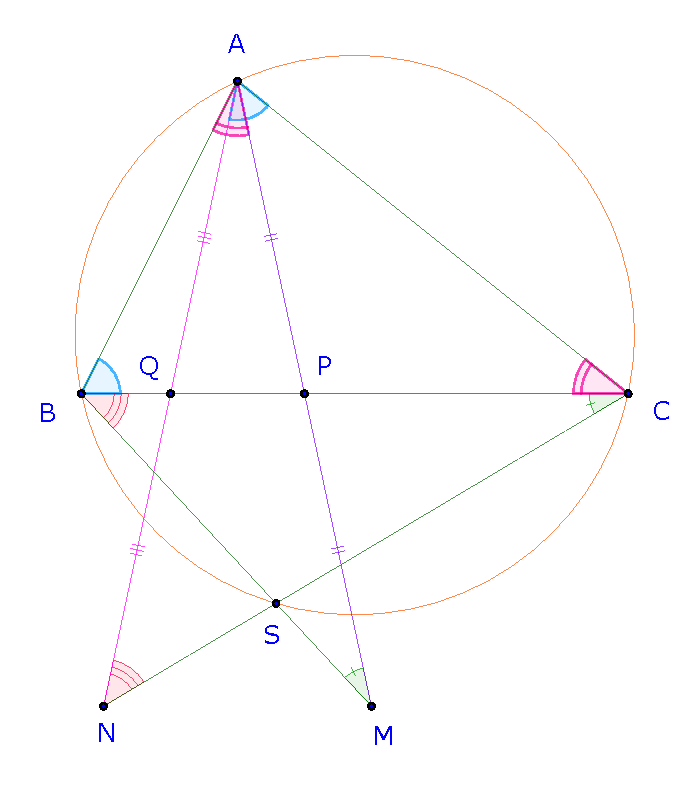
\includegraphics[width=7.5cm]{./svg/pdf/ot-22-23-4-e2-s1.pdf}
    \end{center}

    Now, $\triangle ABC \sim \triangle PBA,$ $ABC$ is anti-clockwise, while $PBA$ is clockwise, thus
    they have different orientations, therefore
    \[
        \frac{A-P}{B-P} = \overline{ \left(\frac{C-A}{B-A}\right) } \quad (1)
    \]

    Similarly 
    \[
        \frac{C-Q}{A-Q} = \overline{ \left(\frac{C-A}{B-A}\right) } \quad (2)
    \]

    But $P$ and $Q$ are midpoints of $AM$ and $AN,$ respectively, thus
    \[
        (3) \quad 
        \begin{cases} 
            &M- P = -(A-P)\\
            &N-Q = -(A-Q)\\
        \end{cases}
    \]

    From (1), (2), and (3) 
    \[
        \frac{M - P}{B -P} = \frac{C- Q}{N- Q}, \text{ thus } \triangle MPB \sim \triangle CQN.
    \]

    From here it is easy to see that $\angle BSC + \angle A = 180\dg,$ thus $BM \cap CN \in (ABC).$
\end{proof}

\end{document}